\chapter{Maximum independent set formulation of the partial row/column assignment problem} \label{chap:independent_set}

With the framework introduced in Section \ref{sec:hot_restart}, we basically translated the problem of the assignment of nonzeros to $A_r$ and $A_c$ (which is already another formulation of the matrix partitioning problem with the medium grain model) to the problem of an efficient computation of a permutation of the indices $0,\dots,m+n-1$. In this chapter, we will propose a method for this vector computation problem, which relies on concepts of the field of graph theory.

The main idea is somewhat similar to the principle that lead us to the development of the Separated Block Diagonal form of order 2 in Section \ref{sec:sbd2}. In that particular form of a partitioned matrix, as already argued, the blocks $\ddot{A}_{00}$ and $\ddot{A}_{44}$ are interesting, because they contain ``independent'' nonzeros. More specifically, those rows and columnsare fully assigned to a processor and whose nonzeros do not have any neighbor (a nonzero in the same row or column) which had a cut column/row. These nonzeros, then, can be assigned anywhere and do not cause communication.

The term \emph{independent}, in this reasoning, has to be defined very carefully: we want to look for a subset of the indices $\{0,\dots,m+n-1\}$ which does not cause any communication, whenever we fully assign its rows to $A_r$ and its columns to $A_c$. With this definition, our goal is clear: we want to assign as much nonzeros as possible in this way, obtaining a low upper bound on the communication volume, which can be computed during the creation of $A_r$ and $A_c$.

To do so, we can employ a very well studied object in graph theory: the \textbf{maximum independent set}. However, this requires a correct translation of our sparse matrix into a graph, described in Section \ref{sec:is_graph}. In Section \ref{sec:is_comp}, instead, we discuss the actual algorithm used to compute the maximum independent set in such graph.

\section{Graph construction} \label{sec:is_graph}

We need to construct the graph correctly from our sparse matrix, in order to retrieve our desired information. In our case, we can simply consider the graph whose adjacency matrix is none other than the sparsity pattern of our matrix $A$. This exact same formulation has already been studied, for the matrix partitioning problem, under the name of \emph{bipartite graph model} by Hendrickson and Kolda \cite{hendrickson}; in the same work, the authors, after constructing the graph, discuss different algorithms for bipartite graph partitioning and come to the conclusion that the best strategy is using multilevel methods with Fiduccia-Mattheyses refinement.

More explicitly, in this graph formulation, we have that rows and columns are vertices, and we have an edge $(i,j)$ if $a_{ij} \neq 0$. It is fairly clear that the resulting graph is bipartite, because an edge connects only rows with columns.

An example of such translation from matrix to graph is shown in Figure \ref{fig:bipartite_graph}, where we start from the matrix given in Figure \ref{fig:partition}. 

\begin{figure}[h]
	\centering
	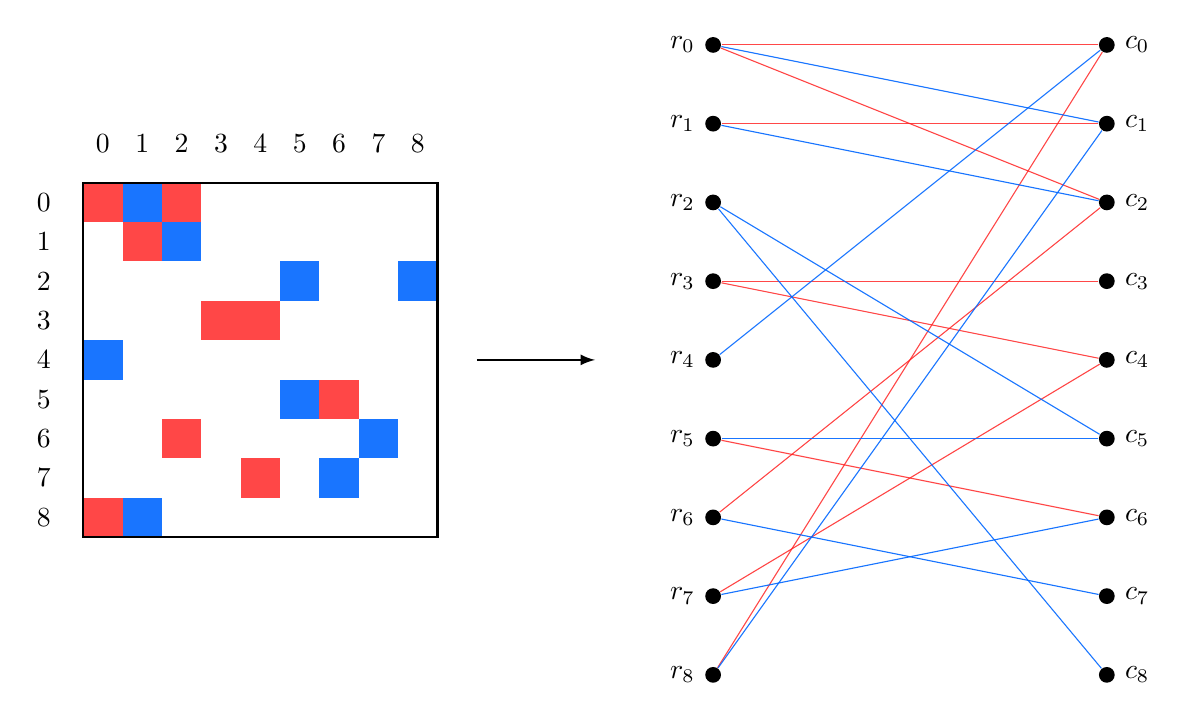
\begin{tikzpicture}[scale=0.5]
		\tikzstyle{myred}=[red!90,opacity=.8]
		\tikzstyle{myblue}=[blue!60!cyan,opacity=.9]
		\tikzstyle{mypurple}=[purple!80!blue,opacity=.9]
		\tikzstyle{myarrow}=[line width=1.3pt,>=latex,->]
		\tikzstyle{vertex} = [fill,shape=circle,node distance=100pt,minimum size=0.2cm,inner sep = 0pt]
		\foreach \x / \y in {1/1,1/3,2/2,4/5,4/4,7/3,8/5,6/7,9/1} { \fill[myred] ({\y-1},{-\x+1}) rectangle +(1,-1);}
		\foreach \x / \y in {1/2,2/3,3/6,3/9,6/6,5/1,7/8,8/7,9/2} { \fill[myblue] ({\y-1},{-\x+1}) rectangle +(1,-1);}
%		\draw[semithick] (0,-9) grid (9,0);
		\draw[thick] (0,-9) rectangle (9,0);

		\draw[myarrow,thick] (10,-4.5) -- (13,-4.5);

		\foreach \x in {0,...,8} { 
			\node[vertex,label=left:\(r_{\x}\)] (r\x) at (16,{3.5-2*\x}) {}; 
			\node[vertex,label=right:\(c_{\x}\)] (c\x) at (26,{3.5-2*\x}) {};
			\node at (-1,{-\x-0.5}) {\x};
			\node at (\x+0.5,1) {\x};
		}

			\foreach \x / \y in {0/0,0/2,1/1,3/4,3/3,6/2,7/4,5/6,8/0} { \draw[myred] (r\x) -- (c\y);}
			\foreach \x / \y in {0/1,1/2,2/5,2/8,5/5,4/0,6/7,7/6,8/1} { \draw[myblue] (r\x) -- (c\y);} 
		\end{tikzpicture}
		\caption{Graph constructed using the sparsity pattern of the matrix of Figure \ref{fig:partition} as adjacency matrix (rows and columns are vertices, nonzeros are edges). The edge color is the same of the corresponding nonzero, but only to facilitate the understanding of this translation; in reality there is no distinction between edges. In the bipartite graph, with $r_i$ we denote row $i$, whereas with $c_j$ we denote column $j$.} \label{fig:bipartite_graph}
	\end{figure}

\section{The maximum independent set and its computation} \label{sec:is_com}

In this section, we will give an extensive overview of the maximum independent set problem, discuss its complexity and the relation with other famous problems in graph theory, and, lastly, give an efficient algorithm that can be used in our case, with a bipartite graph.

\subsection{Maximum independent set}

The concept of independent set is closely related to the concept of \emph{vertex cover} \cite{np_book}: let $G=(V,E)$ be a graph.

\begin{definition}[Independent set]
An \emph{independent set} is a subset $V' \subseteq V$ such that $ \forall u,v \in V'$, $(u,v) \notin E$.
The \emph{maximum} independent set is the independent set of $G$ with maximum cardinality.
\end{definition}

\begin{definition}[Vertex cover]
A \emph{vertex cover} is a subset $V' \subseteq V$ such that $\forall (u,v) \in E$ we have $u \in V' \vee v \in V'$, i.e. at least one of the endpoint of any edge is in the cover.
\end{definition}

\begin{lemma} 
 \label{lemma:is}
 Given a graph $G$, $V'$ is a vertex cover set if and only if $V \setminus V'$ is a independent set.
 \end{lemma}
 \begin{proof}
	 Let $V'$ be a vertex cover, i.e. $\forall (u,v) \in E$, we have that $u \in V'$ or $v \in V'$. This is equivalent to say that $\forall (u,v) \in V \setminus V'$ we have that $(u,v) \notin E$, which is the definition of independent set.
 \end{proof}
As the decision variant of the problem of finding a vertex cover is NP-complete \cite[Theorem 3.3]{np_book}, it follows from this lemma that also finding an independent set in a graph is NP-Complete; the main consequence of this result is that we cannot solve this problem directly for a generic graph, as it would be as hard as our original matrix partitioning problem. Luckily, we are dealing with a particular kind of graph, which simplifies greatly the complexity of the computation of the maximum independent set.

Before exploiting the bipartiteness of our graph, we need to make an additional observation: Lemma \ref{lemma:is} states that the vertex cover problem and independent set cover are complementary. Therefore, computing the maximum independent set is equivalent to computing the minimum vertex cover.

This is particularly useful in our case, because we can use the fact that our graph is bipartite and employ K\H{o}nig's theorem \cite{konig}, which states that, in any bipartite graph, the size of the maximum matching is the size of the minimum vertex cover.

Therefore, it suffices to find an efficient algorithm for the computation of the maximum matching on a bipartite graph, then finding the minimum vertex cover and finally, by taking the complementary set, obtaining the maximum independent set.

\subsection{The Hopcroft-Karp algorithm for bipartite graphs}

